%
\hsection{Reports}%
\label{sec:factory:reports}%
\FloatBarrier%
%
\begin{figure}%
\centering%
%
\subfloat[][%
We select \menu{Reports} in the \menu{Database} pane and click on \inQuotes{Use Wizard to Create Report\dots}%
\label{fig:factoryLibreOfficeBaseReport01main}%
]{\tightbox{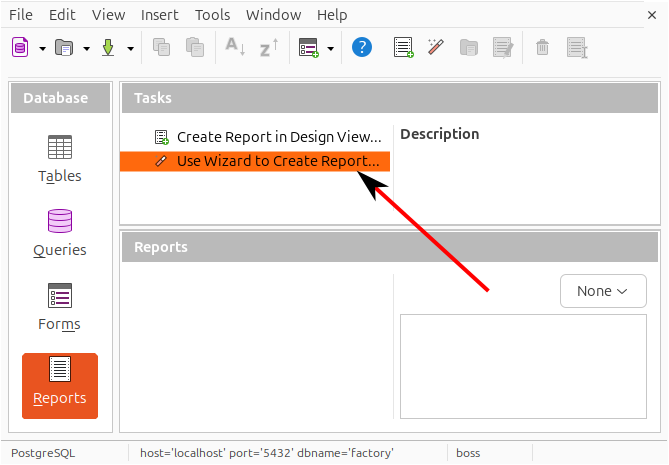
\includegraphics[width=0.49\linewidth]{\currentDir/factoryLibreOfficeBaseReport01main}}}%
%
\floatSep%
%
\subfloat[][%
We need to choose the data source for the new report. %
We click on \inQuotes{Tables \underline{o}r queries.}%
\label{fig:factoryLibreOfficeBaseReport02wizardDataSource}%
]{\tightbox{\includegraphics[width=0.49\linewidth]{\currentDir/factoryLibreOfficeBaseReport02wizardDataSource}}}%
%
\floatRowSep%
%
\subfloat[][%
In the table list that pops up, we scroll down all the way an select \inQuotes{Table: public.sale.}%
\label{fig:factoryLibreOfficeBaseReport03wizardDataSource}%
]{\tightbox{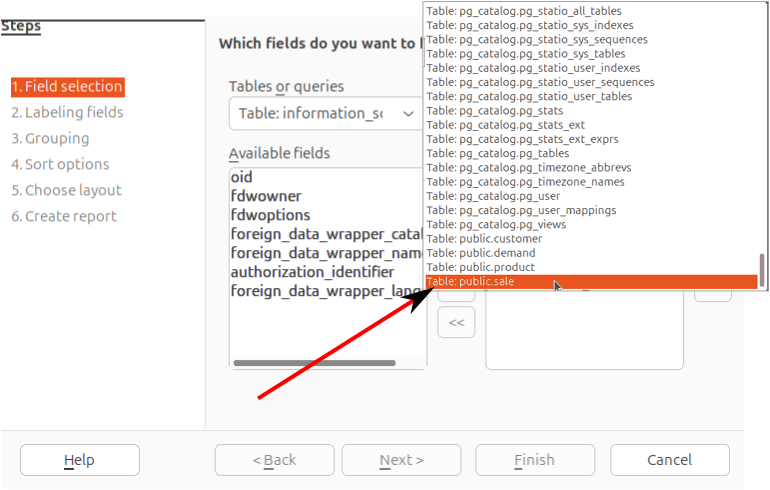
\includegraphics[width=0.49\linewidth]{\currentDir/factoryLibreOfficeBaseReport03wizardDataSource}}}%
%
\floatSep%
%
\subfloat[][%
We get shown all the available columns and select them all. %
Then we click the double greater-than button \menu{\textgreater\textgreater} to add them to the \inQuotes{Fields in report} pane.%
\label{fig:factoryLibreOfficeBaseReport04wizardDataFields}%
]{\tightbox{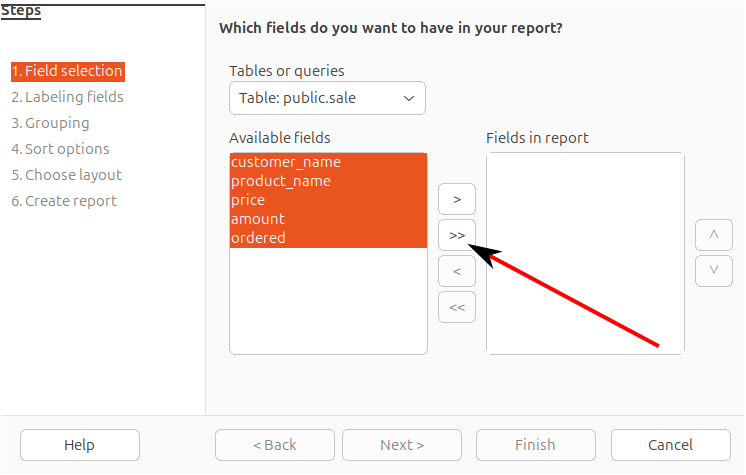
\includegraphics[width=0.49\linewidth]{\currentDir/factoryLibreOfficeBaseReport04wizardDataFields}}}%
%
\floatRowSep%
%
\subfloat[][%
Now that the columns are set up, we click \menu{Next}.%
\label{fig:factoryLibreOfficeBaseReport05wizardDataFieldsChosen}%
]{\tightbox{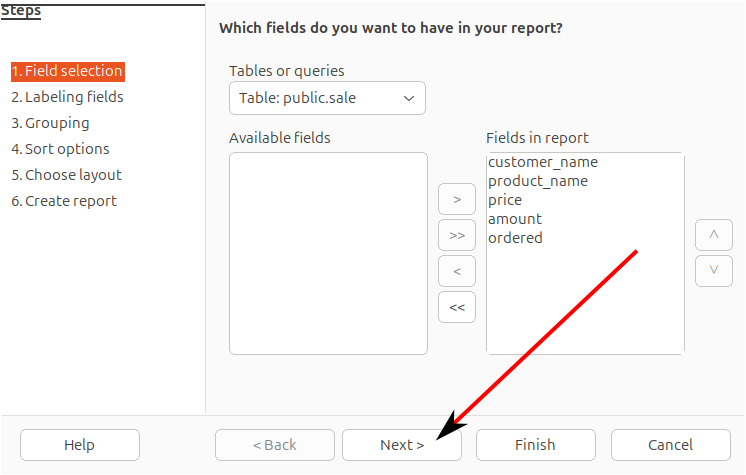
\includegraphics[width=0.49\linewidth]{\currentDir/factoryLibreOfficeBaseReport05wizardDataFieldsChosen}}}%
%
\floatSep%
%
\subfloat[][%
We get asked how we want to label the fields. %
We will enter some more appropriate names.%
\label{fig:factoryLibreOfficeBaseReport06wizardLabels}%
]{\tightbox{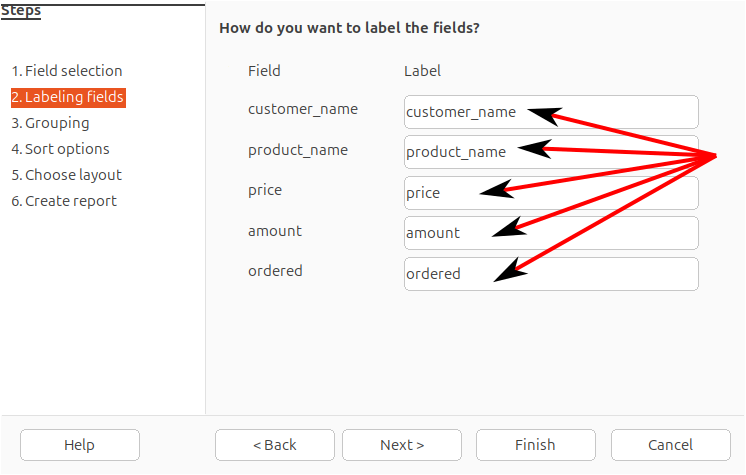
\includegraphics[width=0.49\linewidth]{\currentDir/factoryLibreOfficeBaseReport06wizardLabels}}}%
%
\caption{Creating and executing \db\ reports in \libreofficeBase.}%
\label{fig:factoryLibreOfficeBaseReportA}%
\end{figure}%
%
%
\begin{figure}%
\ContinuedFloat%
\centering%
%
\subfloat[][%
We have chosen more appropriate labels and click \menu{Next}.%
\label{fig:factoryLibreOfficeBaseReport07wizardLabelsChosen}%
]{\tightbox{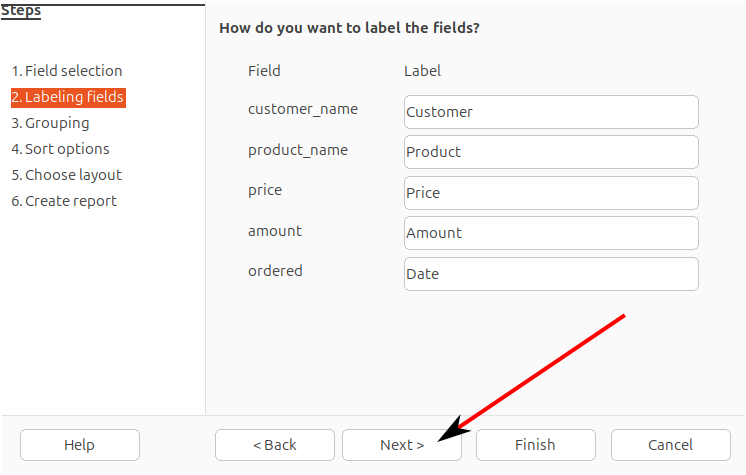
\includegraphics[width=0.49\linewidth]{\currentDir/factoryLibreOfficeBaseReport07wizardLabelsChosen}}}%
%
\floatSep%
%
\subfloat[][%
We now can divide the data into groups. %
We want to divide it into one section per customer in \menu{Fields}. %
So we select \sqlil{customer_name} and click the greater-than button \menu{\textgreater} to move it to \menu{Groupings}.%
\label{fig:factoryLibreOfficeBaseReport08wizardGrouping}%
]{\tightbox{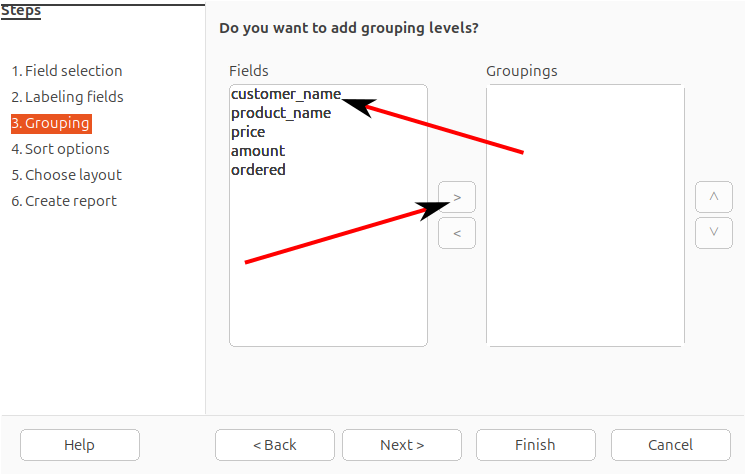
\includegraphics[width=0.49\linewidth]{\currentDir/factoryLibreOfficeBaseReport08wizardGrouping}}}%
%
\floatRowSep%
%
\subfloat[][%
It appears in \menu{Groupings}. %
We click \menu{Next}.%
\label{fig:factoryLibreOfficeBaseReport09wizardGroupingByCustomer}%
]{\tightbox{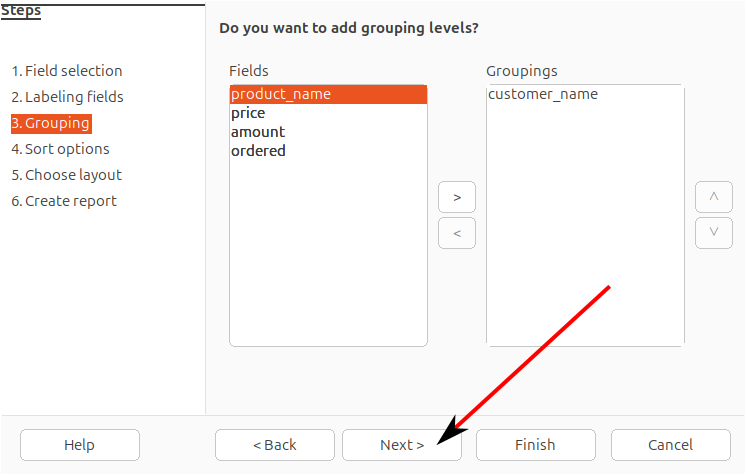
\includegraphics[width=0.49\linewidth]{\currentDir/factoryLibreOfficeBaseReport09wizardGroupingByCustomer}}}%
%
\floatSep%
%
\subfloat[][%
Now we can sort the data records. %
They will already be sorted and grouped by customer. %
However, but inside the customer sections, we want to order the sales demands by date, product~(in case of tied dates), and amount.%
\label{fig:factoryLibreOfficeBaseReport10wizardSorting}%
]{\tightbox{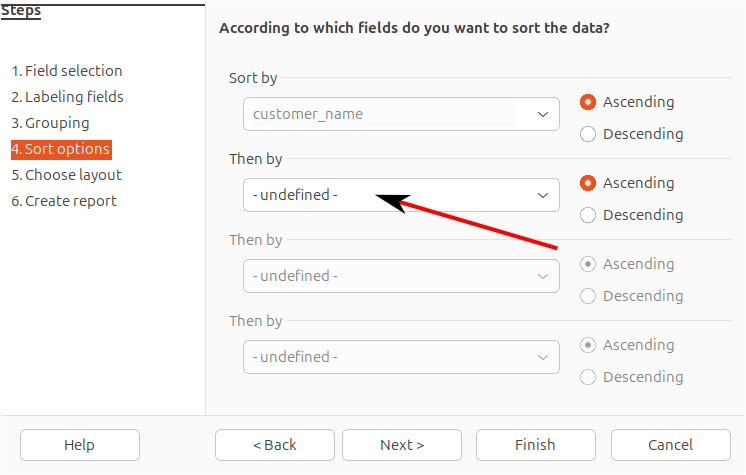
\includegraphics[width=0.49\linewidth]{\currentDir/factoryLibreOfficeBaseReport10wizardSorting}}}%
%
\floatRowSep%
%
\subfloat[][%
We have added the fields. %
Ordering in descending fashion means bigger values first. %
Ordering in ascending fashion means smaller values first. %
We click \menu{Next}.%
\label{fig:factoryLibreOfficeBaseReport11wizardSortingFields}%
]{\tightbox{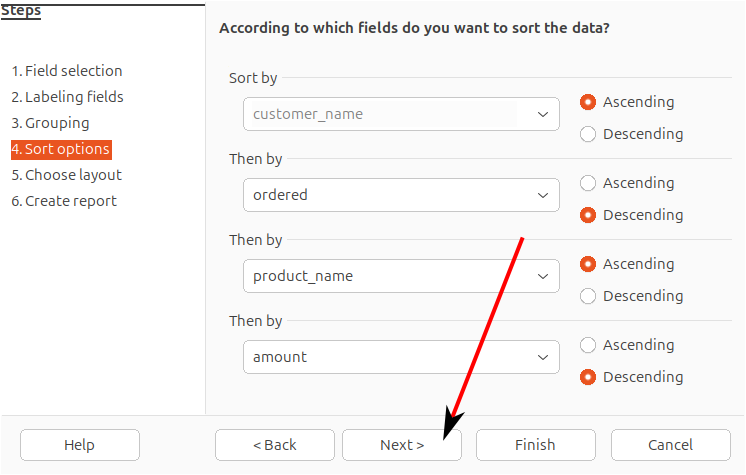
\includegraphics[width=0.49\linewidth]{\currentDir/factoryLibreOfficeBaseReport11wizardSortingFields}}}%
%
\floatSep%
%
\subfloat[][%
We can now choose the layout. %
We are OK with the standard tabular look, but want the report be in portrait format.%
\label{fig:factoryLibreOfficeBaseReport12wizardLayout}%
]{\tightbox{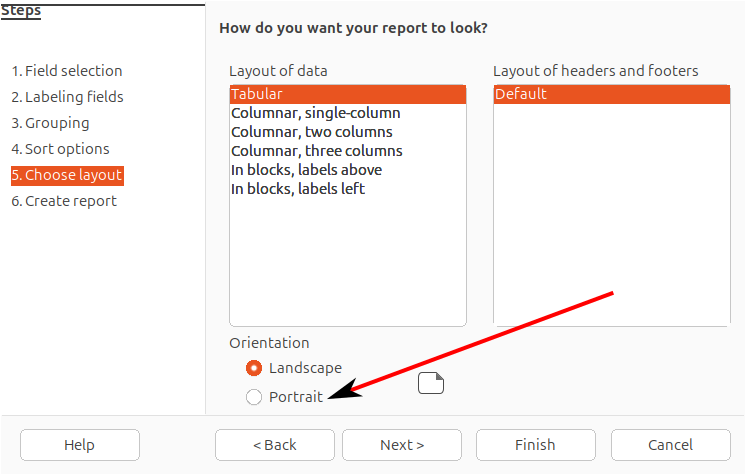
\includegraphics[width=0.49\linewidth]{\currentDir/factoryLibreOfficeBaseReport12wizardLayout}}}%
%
\caption{Creating and executing \db\ reports in \libreofficeBase~(continued).}%
\label{fig:factoryLibreOfficeBaseReportB}%
\end{figure}%
%
%
\begin{figure}%
\ContinuedFloat%
\centering%
%
\subfloat[][%
After changing the layout, we click \menu{Next}.%
\label{fig:factoryLibreOfficeBaseReport13wizardPortrait}%
]{\tightbox{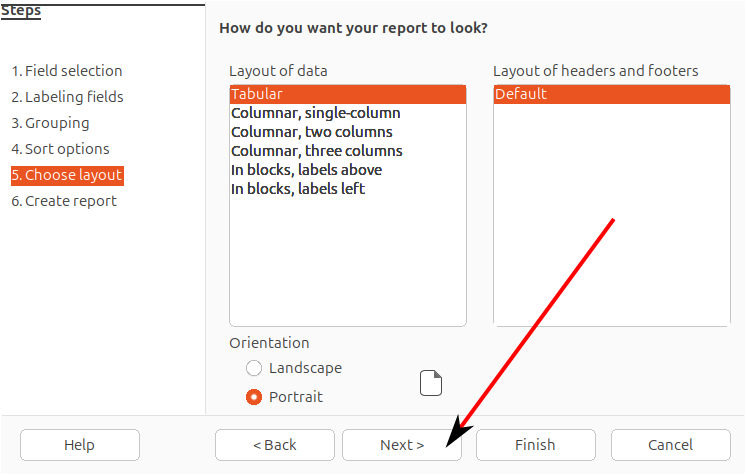
\includegraphics[width=0.49\linewidth]{\currentDir/factoryLibreOfficeBaseReport13wizardPortrait}}}%
%
\floatSep%
%
\subfloat[][%
As report name, we think \sqlil{sale} will be better than \sqlil{public.sale}.%
\label{fig:factoryLibreOfficeBaseReport14wizardCreate}%
]{\tightbox{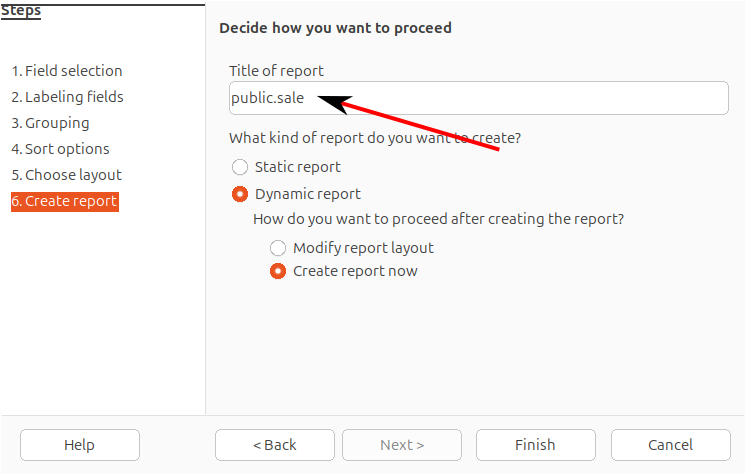
\includegraphics[width=0.49\linewidth]{\currentDir/factoryLibreOfficeBaseReport14wizardCreate}}}%
%
\floatRowSep%
%
\subfloat[][%
We also do not just want to print the report right away, but we want to \inQuotes{Modify report layout.}%
\label{fig:factoryLibreOfficeBaseReport15wizardCreateSale}%
]{\tightbox{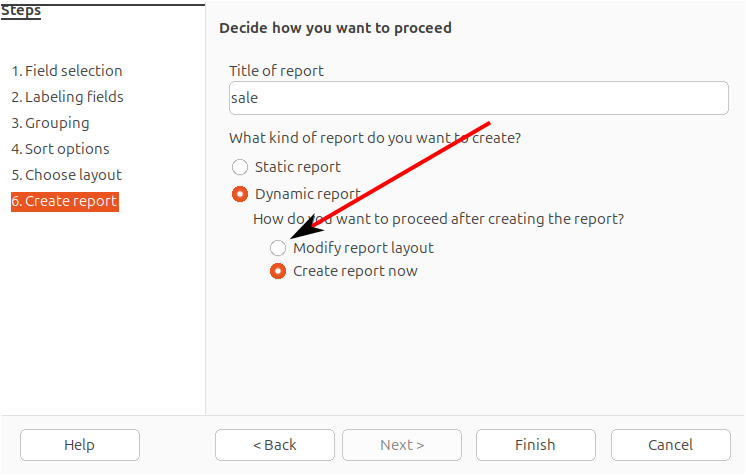
\includegraphics[width=0.49\linewidth]{\currentDir/factoryLibreOfficeBaseReport15wizardCreateSale}}}%
%
\floatSep%
%
\subfloat[][%
We can now click \menu{Next}.%
\label{fig:factoryLibreOfficeBaseReport16wizardCreateModifyLayout}%
]{\tightbox{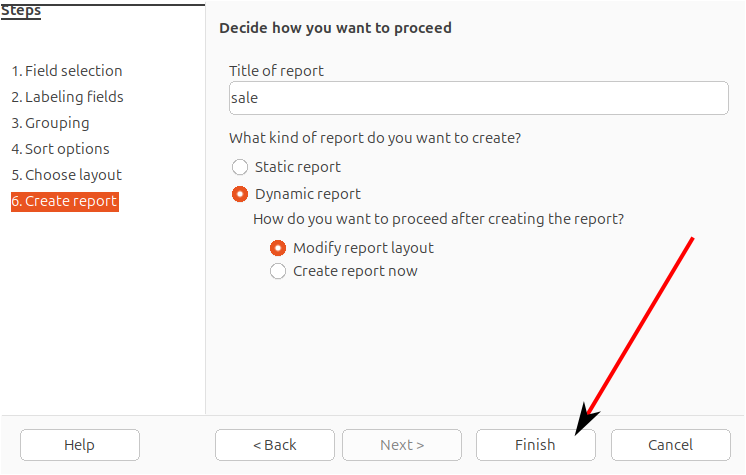
\includegraphics[width=0.49\linewidth]{\currentDir/factoryLibreOfficeBaseReport16wizardCreateModifyLayout}}}%
%
\floatRowSep%
%
\subfloat[][%
The report is created and opened in design view. %
It looks a bit clunky. %
For example, the customer field takes way too much space. %
And it does not need a label. %
So we click the label and press~\keys{\del}.%
\label{fig:factoryLibreOfficeBaseReport17created}%
]{\tightbox{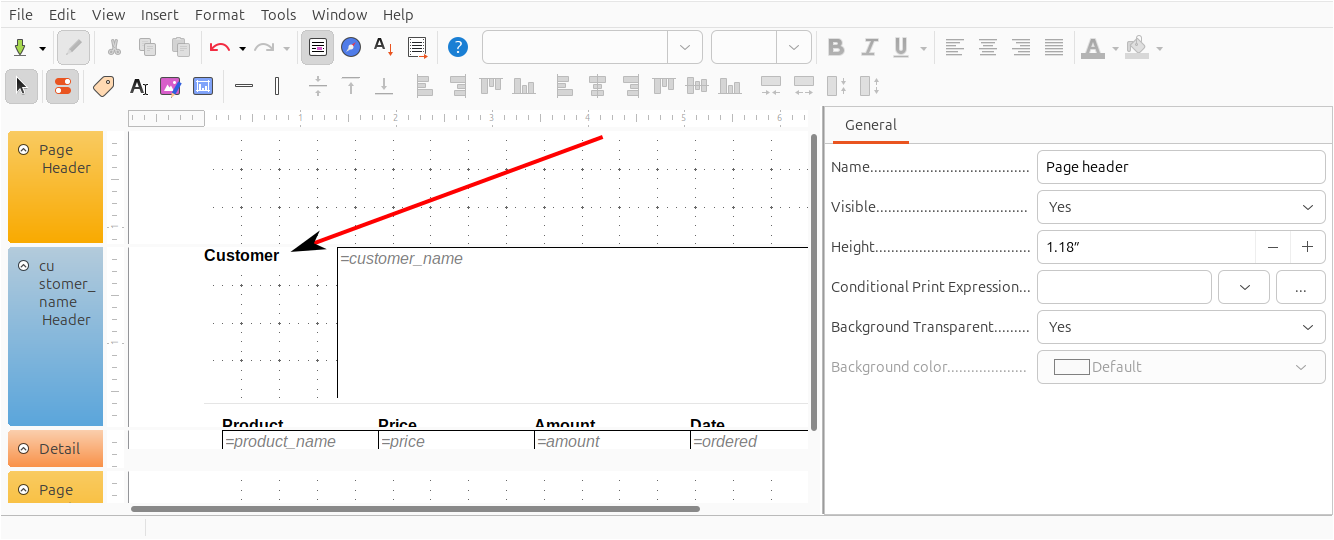
\includegraphics[width=0.49\linewidth]{\currentDir/factoryLibreOfficeBaseReport17created}}}%
%
\floatSep%
%
\subfloat[][%
We also dragged the left corner of the \sqlil{customer} field to the left border. %
We now want to drag its bottom edge up, because it does not need so much space.%
\label{fig:factoryLibreOfficeBaseReport18customerLabelRemoved}%
]{\tightbox{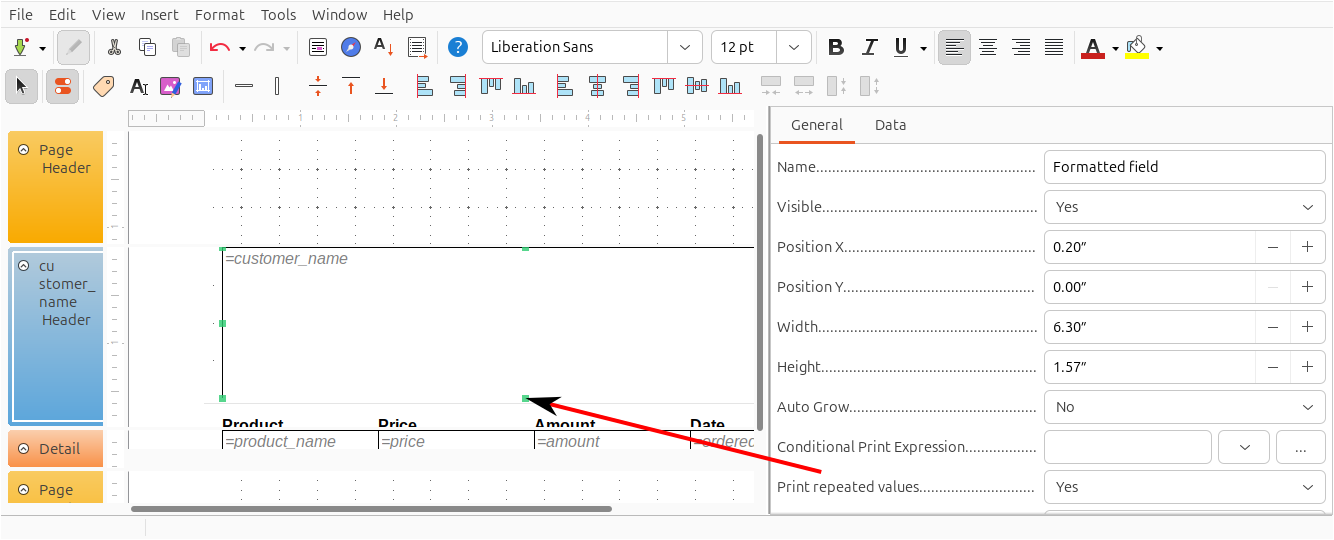
\includegraphics[width=0.49\linewidth]{\currentDir/factoryLibreOfficeBaseReport18customerLabelRemoved}}}%
%
%
\caption{Creating and executing \db\ reports in \libreofficeBase~(continued).}%
\label{fig:factoryLibreOfficeBaseReportC}%
\end{figure}%
%
%
\begin{figure}%
\ContinuedFloat%
\centering%
%
\subfloat[][%
Now it has an appropriate size. %
Next we want to move all the table headers upward.%
\label{fig:factoryLibreOfficeBaseReport19customerShrinked}%
]{\tightbox{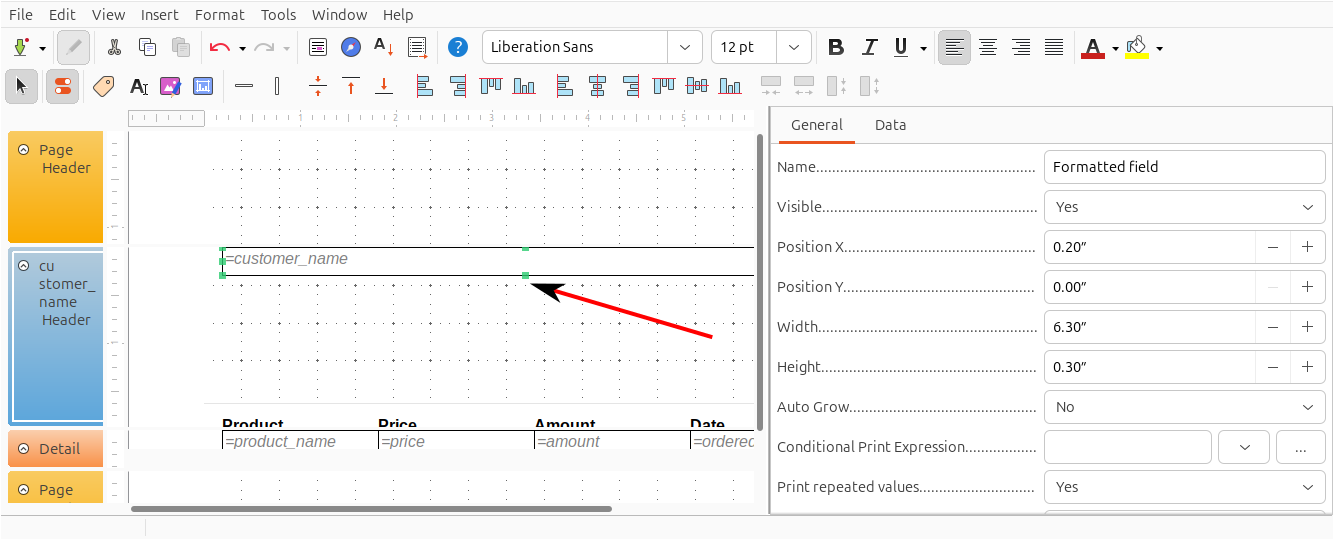
\includegraphics[width=0.49\linewidth]{\currentDir/factoryLibreOfficeBaseReport19customerShrinked}}}%
%
\floatSep%
%
\subfloat[][%
We right-click and drag a selection box around the table header and the horizontal line. %
Then we press the \keys{\arrowkeyup} key a few times to move the header up.%
\label{fig:factoryLibreOfficeBaseReport20headerSelected}%
]{\tightbox{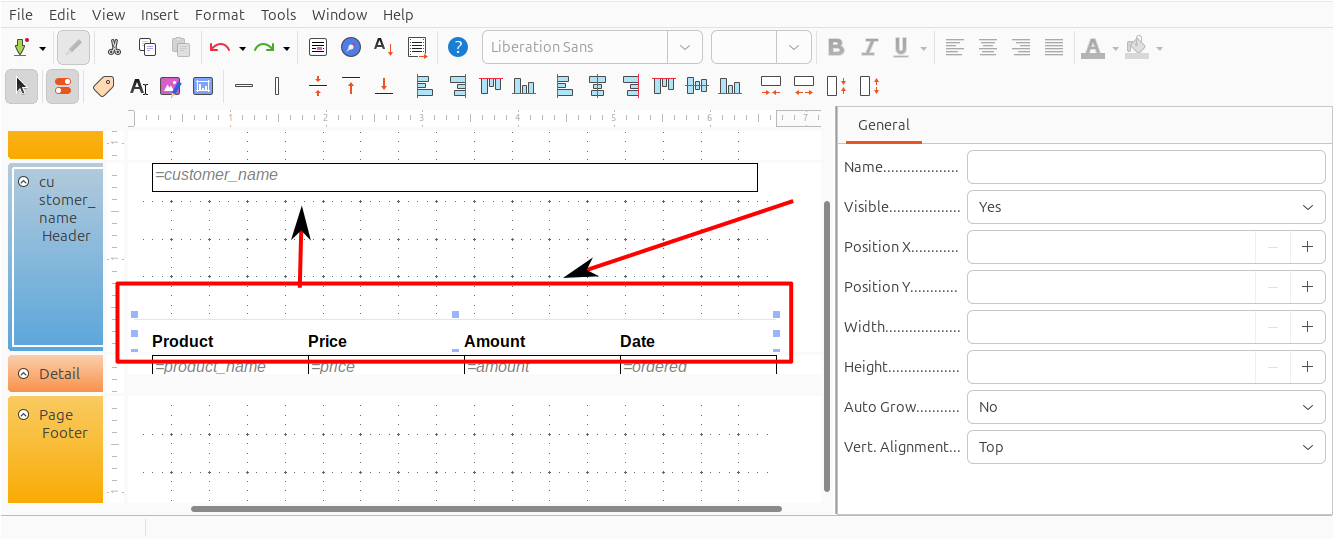
\includegraphics[width=0.49\linewidth]{\currentDir/factoryLibreOfficeBaseReport20headerSelected}}}%
%
\floatRowSep%
%
\subfloat[][%
The header is now moved up.%
\label{fig:factoryLibreOfficeBaseReport21headerMovedUp}%
]{\tightbox{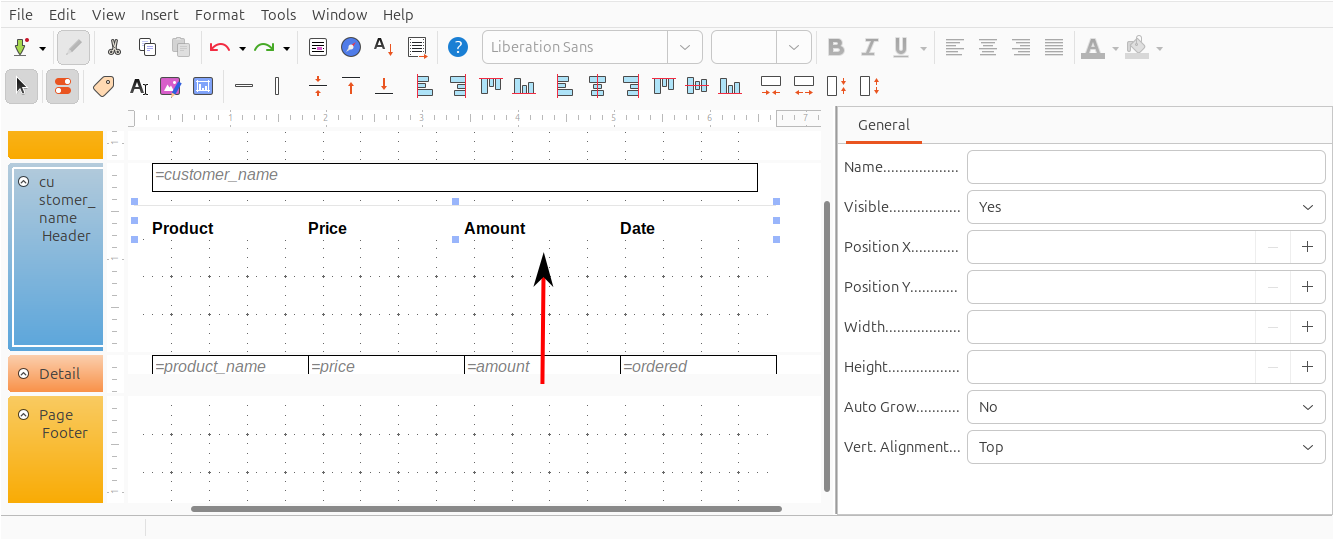
\includegraphics[width=0.49\linewidth]{\currentDir/factoryLibreOfficeBaseReport21headerMovedUp}}}%
%
\floatSep%
%
\subfloat[][%
We now want to make the group header field of the report a bit smaller. %
We click on the \inQuotes{customer\_name Header} pane and then into the \menu{Height} property.%
\label{fig:factoryLibreOfficeBaseReport22headerDeselected}%
]{\tightbox{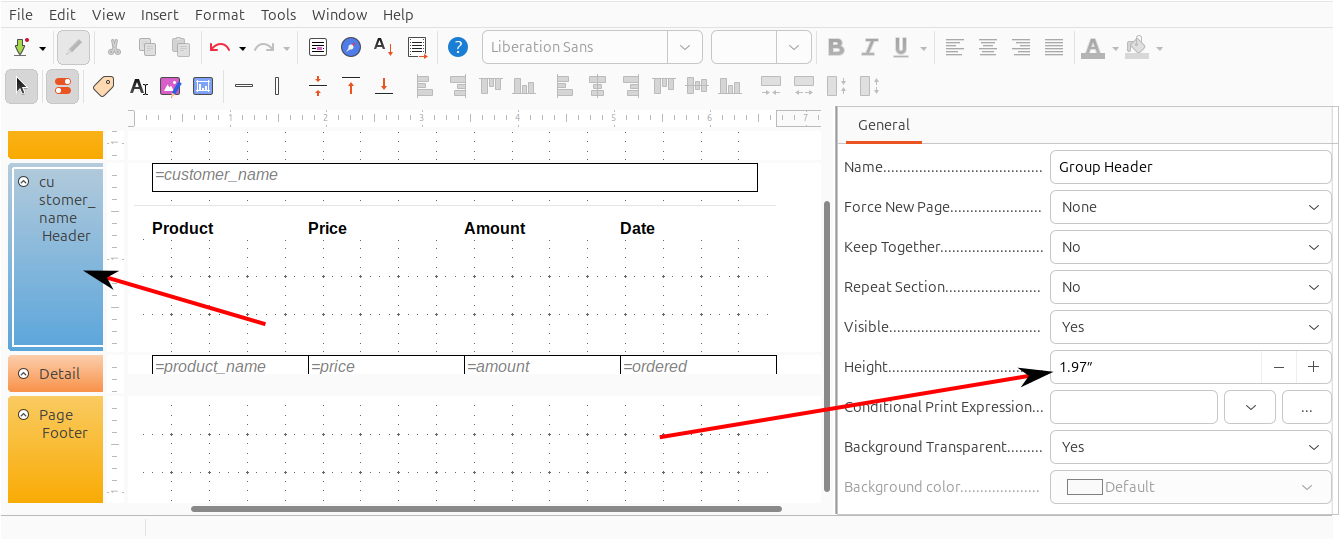
\includegraphics[width=0.49\linewidth]{\currentDir/factoryLibreOfficeBaseReport22headerDeselected}}}%
%
\floatRowSep%
%
\subfloat[][%
We make it nice and small. %
Finally, to create some space between customer groups, we want to move all the header controls down a bit again.%
\label{fig:factoryLibreOfficeBaseReport23headerShrunk}%
]{\tightbox{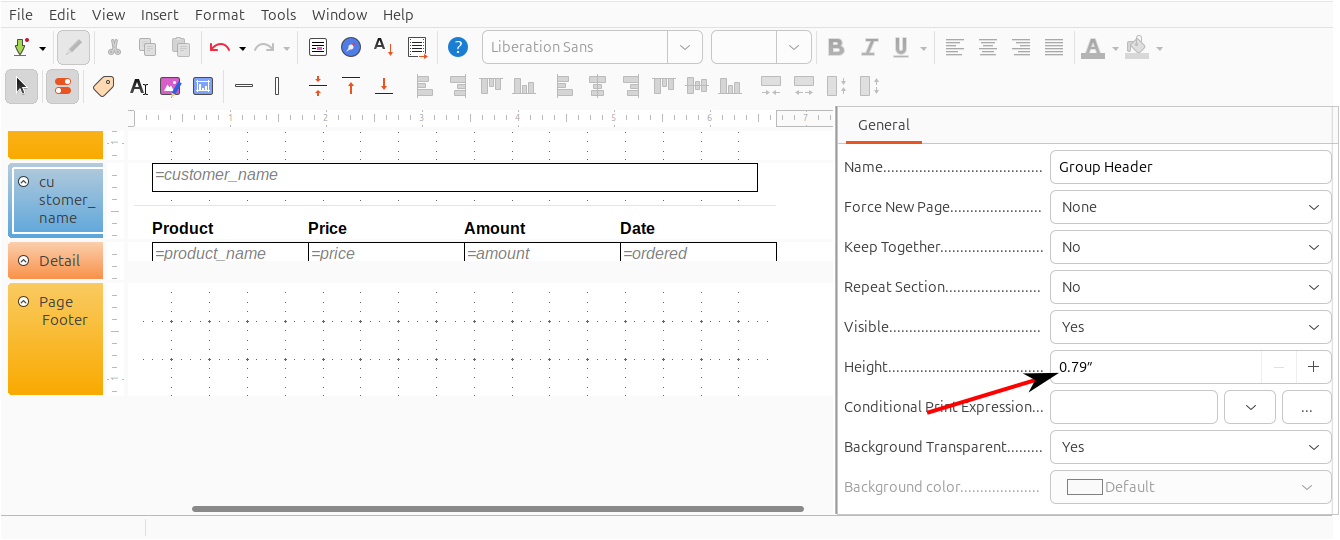
\includegraphics[width=0.49\linewidth]{\currentDir/factoryLibreOfficeBaseReport23headerShrunk}}}%
%
\floatSep%
%
\subfloat[][%
To move them all down, we select them first. %
We right-click into the report and drag a selection box over them.%
\label{fig:factoryLibreOfficeBaseReport24headerSelected}%
]{\tightbox{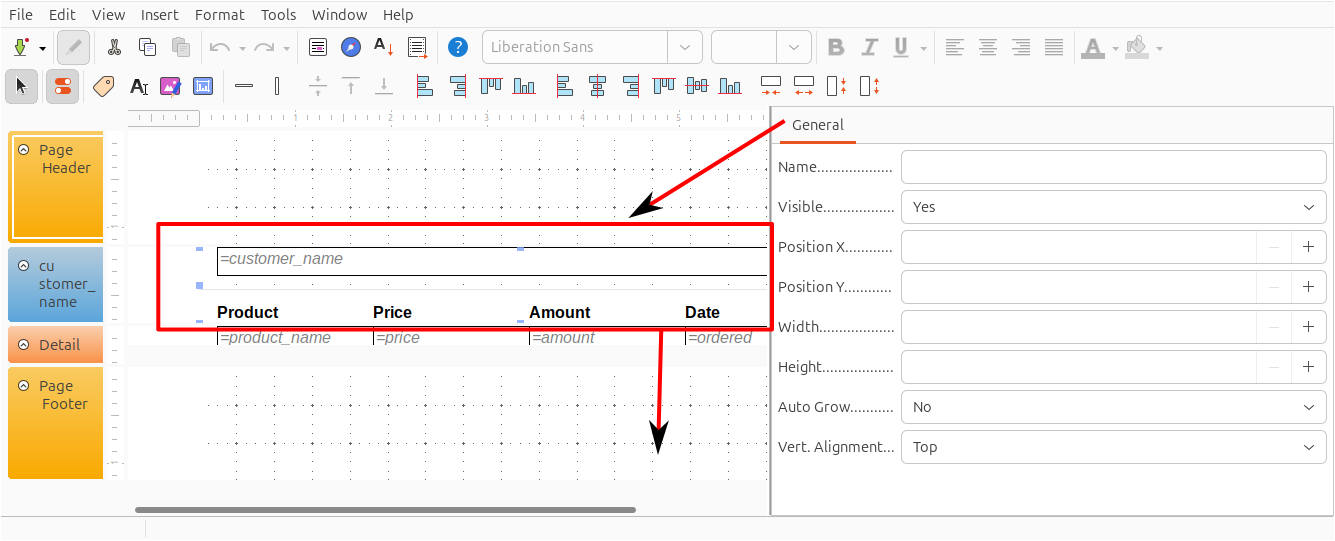
\includegraphics[width=0.49\linewidth]{\currentDir/factoryLibreOfficeBaseReport24headerSelected}}}%
%
\floatRowSep%
%
\subfloat[][%
Then we press the \keys{\arrowkeydown} key a few times. %
We are done and close the report.%
\label{fig:factoryLibreOfficeBaseReport25headerMovedDown}%
]{\tightbox{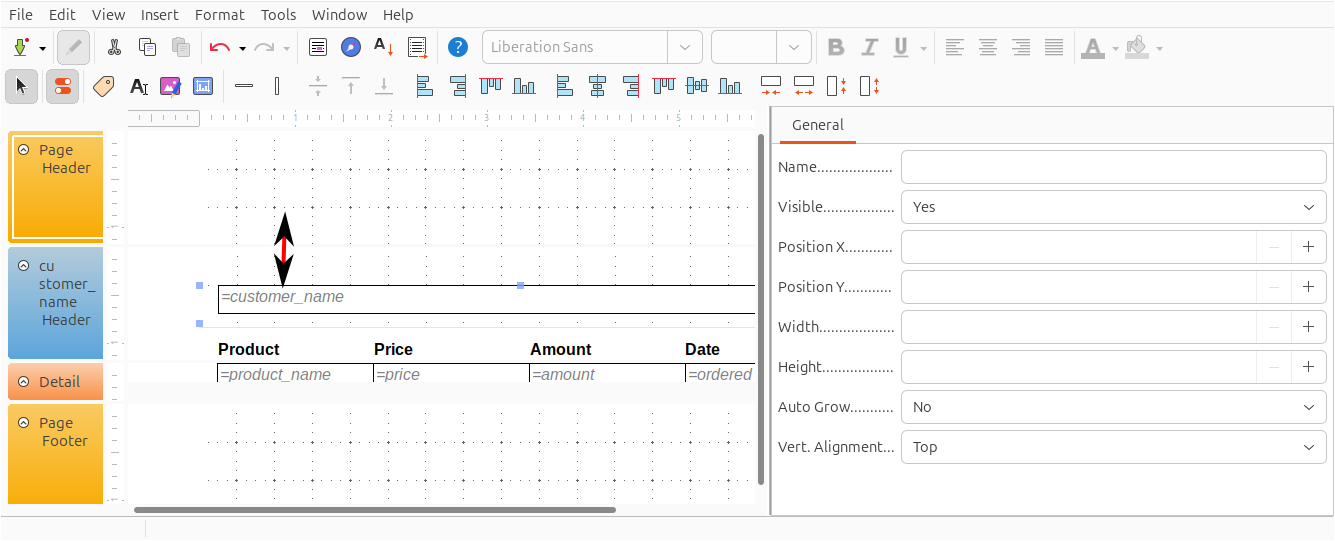
\includegraphics[width=0.49\linewidth]{\currentDir/factoryLibreOfficeBaseReport25headerMovedDown}}}%
%
\floatSep%
%
\subfloat[][%
Upon closing the report, we get asked whether want to save it. %
We click on \menu{save}. %
We save it under the name \textil{sale}.%
\label{fig:factoryLibreOfficeBaseReport26save}%
]{\tightbox{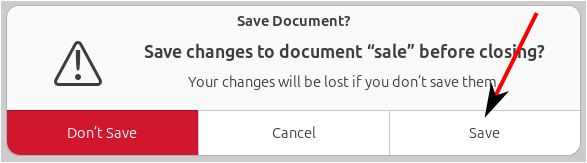
\includegraphics[width=0.49\linewidth]{\currentDir/factoryLibreOfficeBaseReport26save}}}%
%
\caption{Creating and executing \db\ reports in \libreofficeBase~(continued).}%
\label{fig:factoryLibreOfficeBaseReportD}%
\end{figure}%
%
%
\begin{figure}%
\ContinuedFloat%
\centering%
%
\subfloat[][%
And it appears under this name in the \menu{Reports} pane. %
We double-click on it. %
\label{fig:factoryLibreOfficeBaseReport27saved}%
]{\tightbox{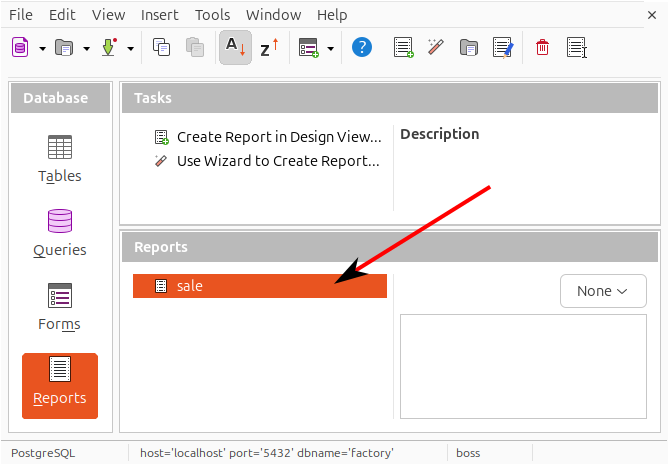
\includegraphics[width=0.49\linewidth]{\currentDir/factoryLibreOfficeBaseReport27saved}}}%
%
\floatSep%
%
\subfloat[][%
A new document opens in \libreofficeWriter. %
It contains all the data in a very nicely formatted fashion. %
We can even export it to \pgls{formatPDF} by clicking the PDF symbol~\libreOfficePdf.%
\label{fig:factoryLibreOfficeBaseReport28executed}%
]{\tightbox{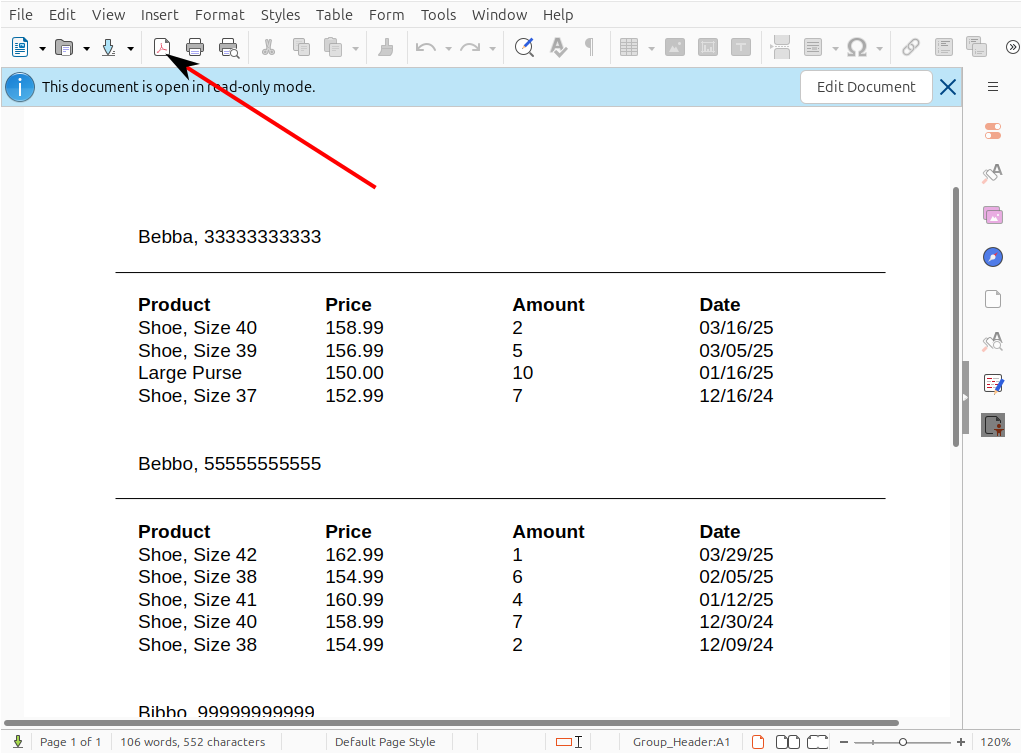
\includegraphics[width=0.49\linewidth]{\currentDir/factoryLibreOfficeBaseReport28executed}}}%
%
\floatRowSep%
%
\subfloat[][%
The exported \pgls{formatPDF} document.%
\label{fig:factoryLibreOfficeBaseReport29report}%
]{\tightbox{\includegraphics[width=0.62\linewidth]{\currentDir/factoryLibreOfficeBaseReport29report}}}%
%
\caption{Creating and executing \db\ reports in \libreofficeBase~(continued).}%
\label{fig:factoryLibreOfficeBaseReportE}%
\end{figure}%
%
%
The last common facette in small-scale \db\ applications that we will consider are \emph{reports}.
A report is basically a nicely-styled document created from the data in a \db.
Forms are a convenient way to enter data into a \db.
Reports are a convenient way to display data from a \db.
If the secretary managing the customer orders wants to compose a overview on the business transactions, then they could look at the output of our view~\sqlil{sale}.
While its output is indeed nicely readable, it is not exactly something that we would print on paper and put on the table of manager.
Now they could copy the data into a \microsoftWord\ document and then print it.
However, this would mean that, everytime such overview is needed, the same copy-paste-format-print workflow needs to be applied.
At the bottom line, reports automate this process.
They offer automated workflows for pre-formatted documents presenting data from a \db.

\libreofficeBase\ also offers the functionality to construct some basic reports.
To explore feature this at least a little bit, first open our dokument \textil{factory.odb} using \libreofficeBase.
To connect with the \db, we will have to enter the password \textil{superboss123}.
Then we select \menu{Reports} in the \menu{Database} pane and click on \inQuotes{Use Wizard to Create Report\dots} in the \libreofficeBase main window as shown in \cref{fig:factoryLibreOfficeBaseReport01main}.

In the dialog that opens up, we need to choose the data source for the new report.
We click on \inQuotes{Tables \underline{o}r queries} in \cref{fig:factoryLibreOfficeBaseReport02wizardDataSource}.
In the table list that pops up, we scroll down all the way an select \inQuotes{Table: public.sale.}
We will use the data from our view~\sqlil{sale}, as shown in \cref{fig:factoryLibreOfficeBaseReport03wizardDataSource}.

In the next step, the dialog shows us all the columns of this view in \cref{fig:factoryLibreOfficeBaseReport04wizardDataFields}.
We select them all and click on the double greater-than button \menu{\textgreater\textgreater} to add them to the \inQuotes{Fields in report} pane.
Now that the columns are set up in \cref{fig:factoryLibreOfficeBaseReport05wizardDataFieldsChosen}, we click \menu{Next}.

Now the dialog asks us how we want to label the fields in \cref{fig:factoryLibreOfficeBaseReport06wizardLabels}.
The column titles of our view are pre-entered for us and while their meaning is clear, text like \sqlil{customer_name} does not look nice in a printed document.
We will enter some more appropriate names.
After choosing some more appropriate labels and click \menu{Next} in \cref{fig:factoryLibreOfficeBaseReport07wizardLabelsChosen}.

The basic building block of a report is a nicely formatted list of all the records in an \sql\ query.
Now the rows can just be printed one by one, or we can structure the report by grouping the data based on the values in certain columns.
In the next step, we can define such a division of the data into groups.
We want to divide the data into one section per customer.
In the \menu{Fields} pane, we select \sqlil{customer_name} in \cref{fig:factoryLibreOfficeBaseReport08wizardGrouping}.
Then, we click the greater-than button \menu{\textgreater} to move it to the \menu{Groupings} pane.
The column now appears in the \menu{Groupings} pane.
We click \menu{Next} in \cref{fig:factoryLibreOfficeBaseReport09wizardGroupingByCustomer}.

The second aspect concerning the linear representation of the data is the ordering.
Since we group the data based on \sqlil{customer_name}, it will automatically be sorted by the customer names.
But we can additionally sort the data based on more columns in \cref{fig:factoryLibreOfficeBaseReport10wizardSorting}.
So our data will be sorted by customer.
However, inside each customer section, it is unsorted.
This does not suit our taste.
We want to order the sales demands by \sqlil{ordered} date.
We want the newest orders to come first, so we will choose descending order.
If multiple demands are issued by a customer on the same date, then we want to break the sorting ties by the \sqlil{product} name~(ordered in ascending fashion).
Any remaining ties should be broken by order amount.
We enter this information in \cref{fig:factoryLibreOfficeBaseReport11wizardSortingFields} and click \menu{Next}.

We can now choose the layout of the report.
We are OK with the standard tabular look, but want the report be in portrait format.
When printing documents \emph{portrait} format means that the format is higher than wide, like the pages in this book.
The \emph{landscape} format pre-selected in \cref{fig:factoryLibreOfficeBaseReport12wizardLayout} format means wider-than-high, i.e., similar how you would paint or take a photo of a landscape.
After changing the layout, we click \menu{Next} in \cref{fig:factoryLibreOfficeBaseReport13wizardPortrait}.

As report name, we think \sqlil{sale} will be better than \sqlil{public.sale} in \cref{fig:factoryLibreOfficeBaseReport14wizardCreate}.
We also do not just want to print the report right away, but we want to \inQuotes{Modify report layout} so we make the corresponding selection in \cref{fig:factoryLibreOfficeBaseReport15wizardCreateSale}.
We can now click \menu{Next} in \cref{fig:factoryLibreOfficeBaseReport16wizardCreateModifyLayout}.

The report is create and opened in design view.
We can see all the controls and data fields placed, but it is not yet clear how the thing will look like when actually printed.
Before we open it, let us make a few small changes to beautify it~(you will thank me later).

Anyway, currently, the report looks a bit clunky.
For example, the customer field takes way too much space.
And it does not need a label.
So we click the label and press~\keys{\del} in \cref{fig:factoryLibreOfficeBaseReport17created}.
The label disappears.
This creates more space on the left side of the \sqlil{customer} field.
So we now also dragged the left corner of the \sqlil{customer} field to the left border of the report.
We now want to drag its bottom edge up, because it does not need so much space in \cref{fig:factoryLibreOfficeBaseReport18customerLabelRemoved}.
Now it has an appropriate size, but lots of useless space is reated below it.

Next we want to move all the table headers upward in \cref{fig:factoryLibreOfficeBaseReport19customerShrinked}.
We therefore right-click and drag a selection box around the table header and the horizontal line.
Then we press the \keys{\arrowkeyup} key a few times to move the header up in \cref{fig:factoryLibreOfficeBaseReport20headerSelected}.
The header is now moved up in \cref{fig:factoryLibreOfficeBaseReport21headerMovedUp}.

We now want to make the group header field of the report a bit smaller.
We therefore click on the \inQuotes{customer\_name Header} pane on the left-hand side.
We then click into the \menu{Height} property in the form on the right in \cref{fig:factoryLibreOfficeBaseReport22headerDeselected}.
We make it value nice and small in \cref{fig:factoryLibreOfficeBaseReport23headerShrunk}.

This, however, will make the report look cluttered because now all the data and groups will stick together.
Finally, to create some space between customer groups, we want to move all the header controls down a bit again.
To move them all down, we select them first in \cref{fig:factoryLibreOfficeBaseReport24headerSelected}.
We right-click into the report and drag a selection box over them.
Then we press the \keys{\arrowkeydown} key a few times.
This creates the needed space in \cref{fig:factoryLibreOfficeBaseReport25headerMovedDown}.
We are done and close the design view of the report.

Upon closing the report, we get asked whether want to save it.
Of course we want to.
We click on \menu{save} in \cref{fig:factoryLibreOfficeBaseReport26save}.

The report now appears under this name in the \menu{Reports} pane.
We double-click on it in \cref{fig:factoryLibreOfficeBaseReport27saved} to finally see how it looks like in action.

A new document opens in \libreofficeWriter.
It contains all the data in a very nicely formatted fashion.
We can even export it to \pgls{formatPDF} by clicking the PDF symbol~\libreOfficePdf\ in \cref{fig:factoryLibreOfficeBaseReport28executed}.
The exported \pgls{formatPDF} document is shown in \cref{fig:factoryLibreOfficeBaseReport29report}.

This looks quite nice.
Of course, we just quickly clicked this report together.
There is much much more that can be done.

Reports often support the ability to compute and present statistics.
We could present the total sales income per customer, for example.
We could just as well as the display overall total income of our company in the report.
It is also often possible to define filters for the data.
We could probably have limited that data to with a start date and end data that the user should enter.

Reports often also allow us to include diagrams.
It is totally possible to include a chart per customer showing when they made purchases and for how much money.
\libreofficeBase\ has this functionality {\dots} but my version of \libreofficeBase\ on computer crashes when I try to use it{\dots}
Well, you can play around a bit and see if you get it to work on your machine.

Either way, the important point is that you now also got to take a glimpse on what reports are in the field of \pglspl{db}.
Reports provide us the ability to automatically generate nicely formatted and pritable views on the data in our \db.
Their output can be understood by people who do not even know what a \db\ is.
Therefore, they are a very common tool in many small and mid-scale applications.
They are supported by tools such as \libreofficeBase\ or \microsoftAccess.
There exist whole software libraries that can generate reports.
For example, there probably are \python\ libraries that can produce beautiful reports, maybe in conjunction with \matplotlib\ and all the other functionality that the \python\ ecosystem can offer us.
And since you already learned how to access a \postgresql\ \db\ from \python, you can also roughly guess how you would get such a report library to work with our \db.%
%
\FloatBarrier%
\endhsection%
%
